\documentclass[10pt]{article}

% amsmath package, useful for mathematical formulas
\usepackage{amsmath}
% amssymb package, useful for mathematical symbols
\usepackage{amssymb}

% graphicx package, useful for including eps and pdf graphics
% include graphics with the command \includegraphics
\usepackage{graphicx}

% cite package, to clean up citations in the main text. Do not remove.
\usepackage{cite}

\usepackage{color} 

% Use doublespacing - comment out for single spacing
\usepackage{setspace} 
\doublespacing

% Text layout
\topmargin 0.0cm
\oddsidemargin 0.5cm
\evensidemargin 0.5cm
\textwidth 16cm 
\textheight 21cm

% Bold the 'Figure #' in the caption and separate it with a period
% Captions will be left justified
\usepackage[labelfont=bf,labelsep=period,justification=raggedright]{caption}

% Use the PLoS provided bibtex style
\bibliographystyle{plos2009}

% Remove brackets from numbering in List of References
\makeatletter
\renewcommand{\@biblabel}[1]{\quad#1.}
\makeatother


% Leave date blank
\date{}

\pagestyle{myheadings}
%% ** EDIT HERE **


%% ** EDIT HERE **
%% PLEASE INCLUDE ALL MACROS BELOW

% figure files reside in the figures/ directory
\graphicspath{
{figures/}
}

%% END MACROS SECTION

\begin{document}

% Title must be 150 characters or less
\begin{flushleft}
{\Large
\textbf{Spatially explicit model of the lymphocyte diaspora in influenza-infected lung quantifies constraints of chemokine directed migration}
}
% Insert Author names, affiliations and corresponding author email.
\\
Drew Levin$^{1,\ast}$, 
Stephanie Forrest$^{1}$, 
Soumya Banerjee$^{1}$
Candice Clay$^{2}$, 
Melanie Moses$^{1}$, 
Frederick Koster$^{2}$, 
\\
\bf{1} Department of Computer Science, University of New Mexico, Albuquerque, NM, USA
\\
\bf{2} Lovelace Respiratory Research Institute, Albuquerque, NM, USA
\\
$\ast$ E-mail: Corresponding drew@cs.unm.edu
\end{flushleft}



% Please keep the abstract between 250 and 300 words
\section*{Abstract}

During the primary immune response clearance of influenza in the lung requires the homing of activated CD8 T cells during the lymphocyte diaspora from regional lymph nodes to small infected foci representing a tiny fraction of the total lung.  T-cell navigation through the complex branching bronchial vascular network is made possible by local cytokine and chemokine production from infected epithelial cells.  Avian H5N1, seasonal H1N1, and 2009 pandemic influenza strains were used separately to induce chemokine production \textit{in vitro}.  Of the eight chemokines tested only CXCL10 (IP-10) and CCL5 (RANTES) were secreted in tissue  (lab results only) with IP-10 always dominating the migration direction.  A delayed differential equation model was fit to the empirical data revealing per cell chemokine production rates for each strain.  These values were coupled with known biological constants to calibrate a spatially explicit agent-based model to explore the effects inter-strain variation of chemokine production on T-cell recruitment.  The spatial nature of the model reveals unique challenges to T-cell recruitment and motility not visible in spatially homogeneous ODE models.  Expanding plaque sizes further isolate infected cells, making T-cell discovery and subsequent clearance of the infection less effective over time.  The immune response is unable to clear the infection of pandemic H1N1 influenza due to the high rate of viral production and plaque size expansion.

% Please keep the Author Summary between 150 and 200 words
% Use first person. PLoS ONE authors please skip this step. 
% Author Summary not valid for PLoS ONE submissions.   
\section*{Author Summary}


\section*{Introduction}

The adaptive immune response induced during an acute influenza A virus infection is a complex web of defense mechanisms able to control all but the most virulent strains.  Understanding all components of defense mechanisms employed will lead to improved vaccine design and strategies to control immunopathology. Elegant studies in the mouse model have described the induction and effector phases of the adaptive immune response, including the functional capabilities of the innate interferon-directed response, macrophages, specific antibody, and cytotoxic effector lymphocytes \cite{Sallusto2000, Joo2008, Mackay2008}.   CD8+ T cells are necessary for the resolution of pneumonia and the complete clearance of mouse-adapted influenza strains \cite{Sallusto2000, Joo2008, Mackay2008, Miao2010}, but gaps remain in our understanding of the behavior of activated T cells in infected tissue.

The generally held view of the sequence of CD8+ T cell events during a primary immune response to influenza in the lung involves the following steps: dendritic cells bearing specific antigen migrate from the lung to the draining lymph node where naïve T and B cell precursors are encountered and activated in specialized architecture \cite{Saenz2010, Beltman2007, Handel2008, Zheng2008, Ingulli2009, Allan1990}.  T cells proliferate in the lymph node and are released into the bloodstream, appearing simultaneous in the lung, spleen and other organs 4-5 days post-infection after to extravasation from the blood, a whole-body distribution known as the lymphocyte diaspora \cite{Thelen2008}.  In the lung, extravasation from capillaries is signaled by inflammatory cytokine-mediated integrin-activation on endothelial cells.  Once in the tissue, T cells are guided up a chemokine gradient to the infected epithelial cell secreting the chemokine.

A number of mathematical models have used detailed mouse model data to abstract the evolution of the immune response and predict its impact on viral kinetics \cite{Thomas-Vaslin2008, Beauchemin2008, Smith2010, Thakar2010, Burrowes2004}.  Such whole-response modeling has considerable potential in selecting the most promising strategies of vaccination and therapy, thus avoiding subsequent expensive animal and human trials.  Models using ordinary differential equations to predict temporal events, however, can not account for the spatial constraints on cell behavior, and therefore make assumptions about the efficiency of each functional component in the model. 

Here we focus on the time and physical constraints of the lymphocyte diaspora using an agent-based model (ABM).  To develop a model with tractable simulations the model does not incorporate some key components of host defense and therefore does not aim to predict the true outcome for each strain examined.   We ask how do very small foci of infected tissue attract limited numbers of activated CD8 T cells after release into the systemic vascular system.  The circulating blood supply services non-infected tissue orders of magnitude larger than the target infected tissue, necessitating an efficient mechanism to focus cell migration.   A host of cytokines and chemokines secreted by infected cells are critical in directing immune cells to sites of infection \cite{Miao2010, Zhao2000, LiJeon2002}.  While each chemokine has been studied in detail for receptor specificity and function in knockout models, the details of chemokine function and efficiency have not been examined in a virus-infected whole animal model.  

To provide data on the local chemokine-secretion environment in which T cells migrate, we used our data on viral secretion and chemokine secretion patterns from human epithelial cells infected in vitro by three different influenza virus strains of avian, seasonal and pandemic origins \cite{Mitchell2011}.   We selected in vitro chemokine data since this tissue environment surrogate may be more accurate than published chemokine levels in mouse blood and bronchial alveolar fluid, and also permits the creation of sustained chemokine gradients within the model lung.  Extensive literature on mouse model data of infections with mouse-adapted strains PR8 and HK-31 were used to populate the ABM model with activated CD8+ T cells. 

The standard hypothesis would posit that in this model the marked strain-specific differences in replication efficiency and tissue spread previously reported \cite{Mitchell2011} would largely determine the outcome of infection as eradication or lack of control.  While we found this to be true, we observed in this spatially explicit model three interesting characteristics of chemokine-directed migration not revealed from experimental data.  First, of the only two chemokines stimulated by all 3 strains, the influence of IP-10 consistently dominated over the effect of RANTES, regardless of strain.  Second, each chemokine exhibited a clear threshold to direct migration, with lesser impact at higher concentrations above the threshold.  Finally, when the search space (infection focus) was large, T cell search became inefficient due to the disappearance of the chemokine gradient and may be reflected in the loss of control of the pandemic strain.  

% You may title this section "Methods" or "Models". 
% "Models" is not a valid title for PLoS ONE authors. However, PLoS ONE
% authors may use "Analysis" 
\section*{Models}


\subsection*{Computational Modeling}

\begin{figure}[ht!]
\begin{center}
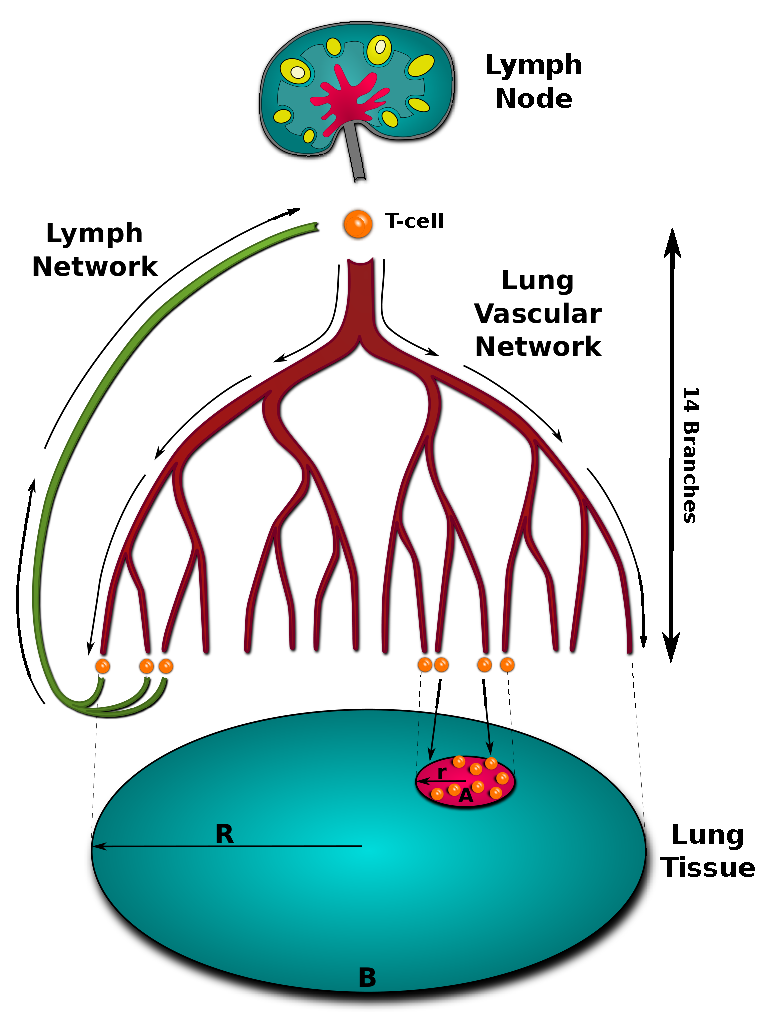
\includegraphics[width=0.4\textwidth]{SystemChart}
\end{center}
\caption{A region of infected tissue of radius $r$ (shaded region $A$) expressing chemokines and inflammatory signals. This region is surrounded by region $B$ which does not have any infected cells and hence does not express either chemokines or inflammatory signals. The $2^{14}$ capillaries (red circles) are distributed evenly throughout the entire lung (region $A$ and $B$).}
\label{fig:systemchart}
\end{figure}

Computational modeling was conducted using CyCells \cite{Warrender2006}, a modeling platform for implementing two- or three-dimensional agent-based simulations of immune response. A simplified model of T-cell activation and recirculation was implemented in CyCells (Fig 1) and simulations were conducted to measure efficiency of infection clearance under different environmental conditions. To model a growing infection, the lung was represented as a two dimensional sheet of healthy epithelial cells. Vasculature was represented as a binary tree with fourteen branches originating at a single lymph node. Activated T-cells descend through the vascular tree until cytokine signal is detected, at which point they exit the vasculature and follow the chemotactic gradient to the site of infection. T-cells that do not encounter cytokine recirculate to the lymph node. Once at the site of infection, a T-Cell may encounter an infected epithelial cell and induce apoptosis.

The simulation begins when a single cell in the center of the tissue is infected. After the eclipse phase (incubation), the infected cell begins secreting virus and chemokine. Virus diffuses locally, infecting nearby cells, and continuing the cycle. The chemokine diffuses from secreting cells, thus increasing the size of the signaling area. After a delay to simulate lymph node stimulation and T-Cell proliferation, activated T-cells begin exiting the lymph node and circulating through the vasculature to the tissue. Because T-Cells cannot choose their path through the branching network, we assume they arrive in tissue at random locations. Figure \ref{fig:modelchart} illustrates the model components 
(epithelial cells, T-cells, and particles) and how they transition between different states.


\subsection*{Model Definition}

\begin{figure}[ht!]
\begin{center}
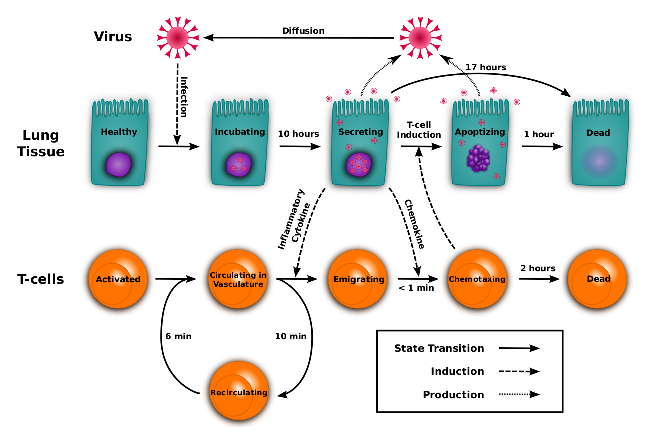
\includegraphics[width=\textwidth]{ModelChart}
\end{center}
\caption{Computational model: Components and state transitions.}
\label{fig:modelchart}
\end{figure}

Epithelial cells are stationary and can be in of five different states: \emph{healthy}, \emph{virus-incubating}, \emph{virus-expressing}, \emph{apoptotic}, and \emph{dead}. \emph{healthy} cells remain unchanged unless infected by virus. Once infected, there is a 10h incubation window before the cell transitions from {incubating} to \emph{expressing}. \emph{Expressing} cells secrete virus and chemokine for 17 hours and then die. \emph{Expressing} cells become \emph{apoptotic} if they encounter activated T-cells. Apoptoic cells continue to secrete virus and die one hour after their transition. \emph{Dead} cells remain inert and do not regenerate over the course of an infection.

T-cells have three states: \emph{searching}, \emph{recirculating}, and \emph{activated}. T-Cells begin emerging from the lymph node at five days post infection at the rate of 777 T-cells per hour for the duration of the simulation. T-Cells enter the vascular system in the \emph{searching} state, arriving at a random location on the lung's surface. \emph{searching} cells perform a random walk in the tissue for 10 minutes, after which they transition to \emph{circulating} if they fail to encounter chemokine. \emph{Circulating} cells spend six minutes recirculating to the lymph node where they are converted to \emph{searching} and reintroduced to a new random location in the lung. If a \emph{searching} T-Cell encounters chemokine, it immedaiately converts to \emph{activated} and begins climbing the chemotactic gradient to the source of infection. \emph{Activated} T-Cells move continuously up the gradient and if they encounter \emph{expressing} epithelial cells, the epithelial cell transitions \emph{apotosis}. Activated T-cells are removed from the simulation using an exponential decay rate with an average lifespan of two hours. 

The model contains two kinds of particles: virus and chemokine. Both are produced at constant rates by \emph{expressing} epithelial cells.  Virus diffuses through the lung tissue, infecting healthy cells probabilistically according to the local virus concentration. Chemokine diffuses across the tissue but has no
direct effect beyond activating T-Cells. Both particle types decay over time.


\subsection*{Parameters}

Define CyCells environment.  Talk about the need for spatial model.  Human/mouse scaling.  Parameter definitions. 

\begin{table}
\begin{tabular}{ | c | c | c | }
  \hline                        
  Paramter & Value & Source \\
  \hline
  Viral Diffusion & .0318 & \cite{Beauchemin2006} \\
  Viral Decay &  $1/day$ & Phenomenological \\
  Chemokine Diffusion & $.318 \mu m^2/s$ & \cite{Beauchemin2006} \\
  Chemokine Decay &  $3.8508e-4/s$ & 30m half-life \\
  Infection Sensitivity &  $2 h/virion$ & Phenomenological \\
  Incubation Time &  $10 h$ & \cite{Mitchell2011} \\
  Expression Time &  $16.7 h$ & \cite{Mitchell2011} \\
  Apoptosis Time & $1 h$ & Phenomenological \\
  T-Cell Production Rate & $777/h$ & \cite{Miao2010} \\ 
  Circulation Time & $6 m$ & \cite{Banerjee2010b} \\
  Search Time & $10 m$ & \cite{Banerjee2010b} \\
  T-Cell Speed (Search) & $30 \mu m/s$ & \cite{Miller2003} \\
  T-Cell Speed (Activated) & $3 \mu m/s$ & \cite{Miller2003} \\
  T-Cell Sensitivity & $1 ng/mL$ & \cite{Gao2003} \\
  T-Cell Expected Kill Rate & $10 m$ & Fred/Drew \\
  Cell Radius & $25 \mu m$ & Phenomenological \\
  T-Cell Age (at FOI) & $2 h$ & [REF] \\
  T-Cell Age (Other) & $3 d$ & [REF] \\
  T-Cell Ramp Up Time & $5 d$ & \cite{Banerjee2011} \\
  IgM Strength & Viral decay of $3/day$ & Phenomenological \\
  \hline  
\end{tabular}
\caption{Generic model parameters}
\label{table:parameters}
\end{table}


\begin{table}
\begin{center}
\begin{tabular}{ | r | c | c | }
  \hline                        
  Paramter & Value & Source \\
  \hline
  IP-10 Production Rate &  & ODE Fits \\
  Avian H5N1 & 2.0e-4 pg/s$\cdot$cell & \\
  Seasonal H1N1 & 1.8e-4 pg/s$\cdot$cell& \\
  Pandemic H1N1 & 8.7e-5 pg/s$\cdot$cell& \\
  \hline
  RANTES Production Rate & & ODE Fits \\
  Avian H5N1 & 1.3e-5 pg/s$\cdot$cell& \\
  Seasonal H1N1 & 8.9e-7pg/s$\cdot$cell& \\
  Pandemic H1N1 & 4.4e-6 pg/s$\cdot$cell& \\
  \hline
  Virus Production Rate &  & \cite{Mitchell2011} \\
  Avian H5N1 & 5.4e-5 PFU/s$\cdot$cell& \\
  Seasonal H1N1 & 3.8e-4 PFU/s$\cdot$cell& \\
  Pandemic H1N1 & 5.1e-3 PFU/s$\cdot$cell& \\  
  \hline  
\end{tabular}
\caption{Strain specific model parameters}
\label{table:strains}
\end{center}
\end{table}

\section*{Materials}

Chemokine secretion:  Epithelial cell culture and supernatant collection was performed as described \cite{Mitchell2011}.  Briefly, undifferentiated human tracheal epithelial cells (University of Miami) were cultured for 4 weeks to achieve fully differentiated confluent monolayers on collagen-coated transwell inserts, or commercial differentiated human bronchial epithelial cells (EpiAirway Tissue, MatTek Corp., Ashland, MA) used immediately upon receipt, were infected at an MOI of 0.01 with either a seasonal H1N1 virus A/New Caledonia/20/99 (sH1N1), the 2009 H1N1 pandemic strain A/California/04/09 (pH1N1), or an avian H5N1 virus A/Hong Kong/483/97 (aH5N1) derived from a fatal human infection.  Apical fluid for viral secretion, and basal media for chemokine secretion collected before treatment of the monolayer with protease, was collected from previously undisturbed triplicate or quadruplicate wells at 0, 6, 10, 12, 16, 20, 24, 30, 36, 42, 48, and 72 hours after infection, and stored at -80C until assay.  Quantitative viral culture was performed by standard plaque assay.  Quantitative chemokine levels were performed in 30 µl aliquots for a panel of 17 chemokines and cytokines (Luminex Assay®, Luminex Corp.) and reported as ng/mL basal media sampled from a total volume of 4 mL.

% Results and Discussion can be combined.
\section*{Results}

\subsection*{Chemokine production}

Chemokine data were collected from epithelial monolayers infected with influenza strains, as described in \cite{Mitchell2011} (Fig.~\ref{fig:data}).  IP-10 concentration increases were observed by 8h p.i., and RANTES by 16h p.i..  To estimate per-cell production rates, we extended the ODE model of Ref. \cite{Mitchell2011} to represent chemokine production from infected cells.  Model fits were generated for three influenza strains (Fig.~\ref{fig:data}) using a genetic algorithm \cite{Mitchell2011}.  The model estimates are shown in Table~\ref{table:strains}.  These expression rates are similar across different strains with the exception of significantly higher RANTES production in aH5N1.  There is no discernible correlation between viral production and induced chemokine production across the three strains of influenza.

\begin{figure}[ht!]
\begin{center}
 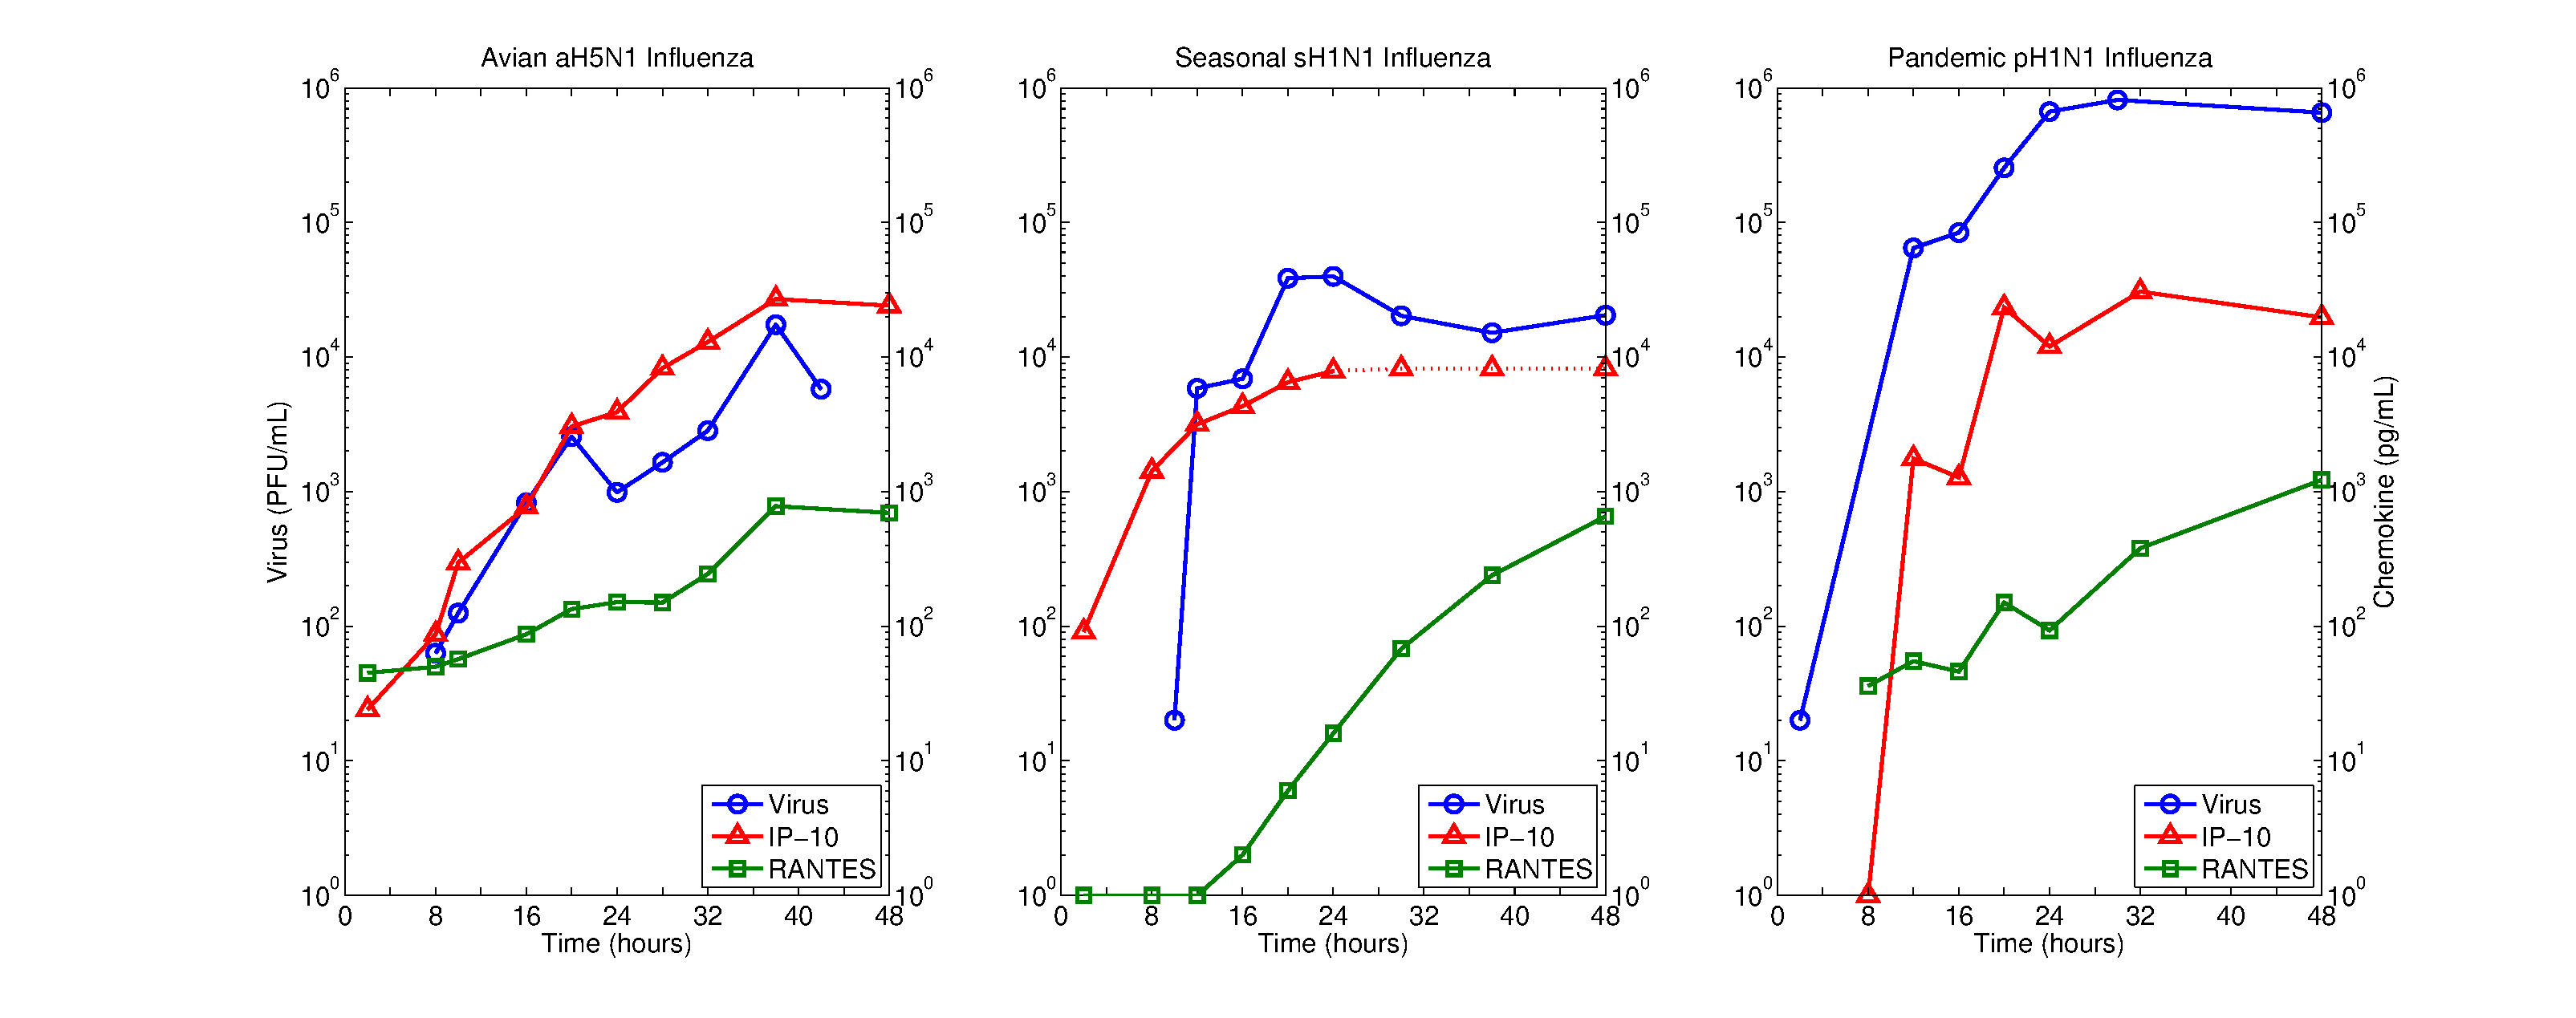
\includegraphics[width=\textwidth]{data}
 \end{center}
\caption{Empirical data of viral and cytokine titer for three strains of influenza: Avian H5N1 (A), Seasonal sH1N1 (B), and Pandemic pH1N1 (C).  For each strain, the viral load (blue circle) is shown in PFU/mL and the chemokines IP-10 (red triangle) and RANTES (green square) are shown in ng/mL.  sH1N1 IP-10 registered three values above the measurement threshold of 8,500 $pg/mL$ (dotted line).  These values were not included in model fitting.} 
 \label{fig:data}
\end{figure}

\subsection*{Stochastic modeling effects}

Unlike ODE models, which are deterministic, stochastic models such as CyCells can produce different results on different runs (Figure~\ref{fig:variance}).  To test the strength of this effect, we ran each model fifty times using the default parameters given in Table~\ref{table:parameters}.  $R^2$ values were calculated for individual runs versus the average of all runs.  Pandemic H1N1 showed the least inter-run variance with an mean $R^2$ value of 0.9935 and standard deviation of 0.0029.  sH1N1 had a mean $R^2$ 0.9859 with a standard deviation of 0.0109.  aH5N1 had a mean $R^2$ of 0.9167 with a standard deviation of 0.0726.  

Each run took the calculated viral production and chemokine production rates for the three different strains of influenza as input and reported the total number of infected cells, including incubating, virus secreting and apoptotic, but not including dead cells.  Therefore the figures approximate plaque growth over time.

Overlaying multiple runs on a single plot reveals a slight growth rate transition 3 days p.i., which reflects the presence of IgM.  In addition, for each infection the number of infected cells declines quickly at day five due to the T-cell response. 

The three strains show different levels of virulence, consistent with the results found in Mitchell (Fig.~\ref{fig:variance}).  The rapid growth of the pandemic H1N1 prevents the immune response from containing the infection.  By the time T-Cells arrive, the plaque is too large for them to cover effectively.  Because pH1N1 is replicates at such a rapid rate, the window of opportunity for T-Cells to gain ground is too small.  aH5N1 is cleared completely, sH1N1 is contained but not fully cleared, and pH5N1 recovers and continues to expand.

\begin{figure}[ht!]
\begin{center}
 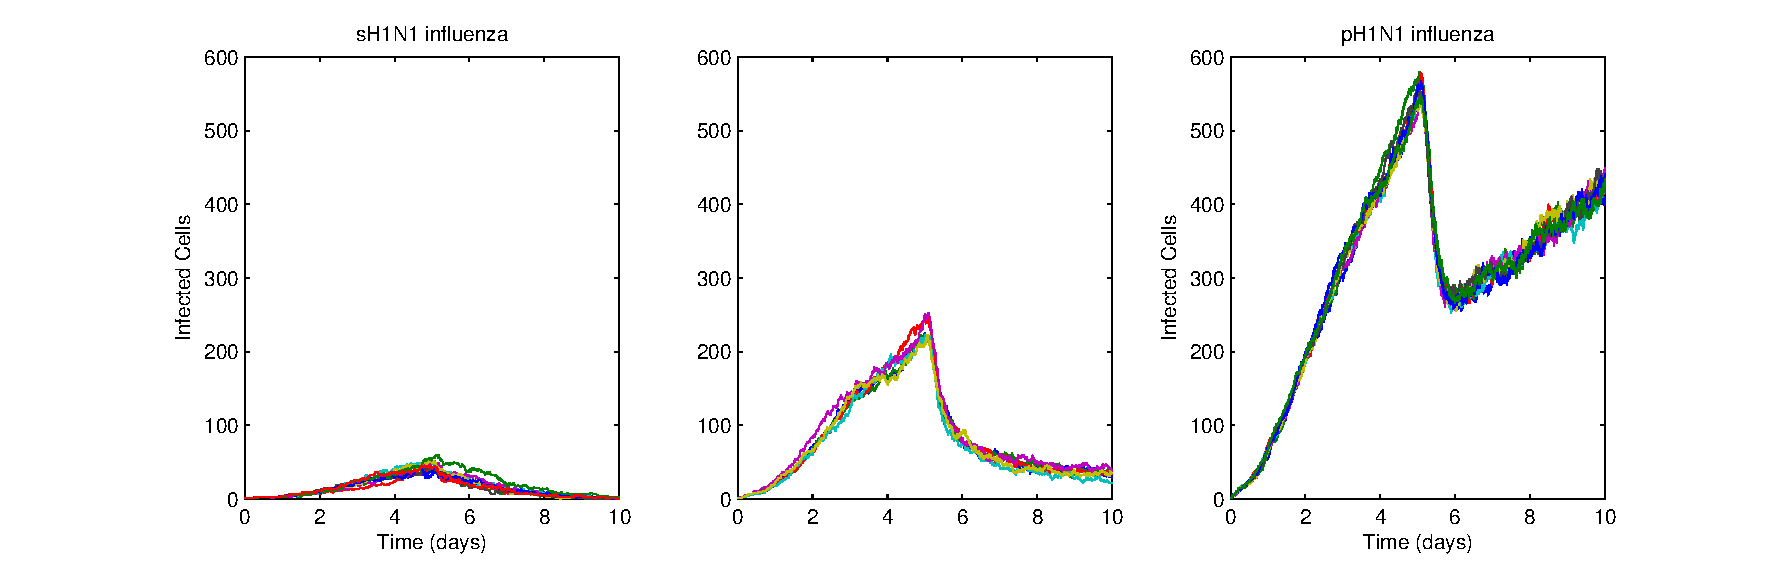
\includegraphics[width=\textwidth]{variance}
 \end{center}
\caption{Model results: Time series plots of fifty runs of aH5N1 (A), sH1N1 (B), and pH1N1 (C) infections (gray). IP-10 and RANTES were simulated in each run, except for aH5N1, which  produced only RANTES.  Each run was initialized identically for each strain.  The middle line shows the average while the outer lines show the 95\% confidence interval.} 
 \label{fig:variance}
\end{figure}


\subsection*{T-cell sensitivity to chemokine}

T-Cells exit a capillary when they sense inflammatory cytokine and then follow the chemokine gradient in tissue.  We use the chemokine gradient as a proxy for the inflammatory response.  Figure \ref{fig:cycells} shows chemokine concentrated around virus secreting cells.  T-cell sensitivity determines how much aggregate chemokine signal is required to detect the gradient.

To test for the minimum concentration of cytokine/chemokine signal required to recruit T-Cells from capillary, we simulated sensitivity levels ranging over seven orders of magnitude. We find a threshold (Fig.~\ref{fig:sensitivity}) between the concentrations of (FIXME: new values) 100 and 10 $ng/ml$, below which there is no discernible effect on infection kinetics.  Because multiple T-cells in the same area do not increase the rate at which apoptosis is induced, we hypothesize that a critical number of T-cells are required to clear an infection above which there is no additional benefit gained from increasing T-cell presence.  Reference \cite{Gao2003} reports T-cell chemotaxis at concentrations as low as 1 $nM$ ($10 ng/mL$ assuming a chemokine weight of $10 kDa$), therefore we use that sensitivity for each model run.

\begin{figure}[ht!]
\begin{center}
 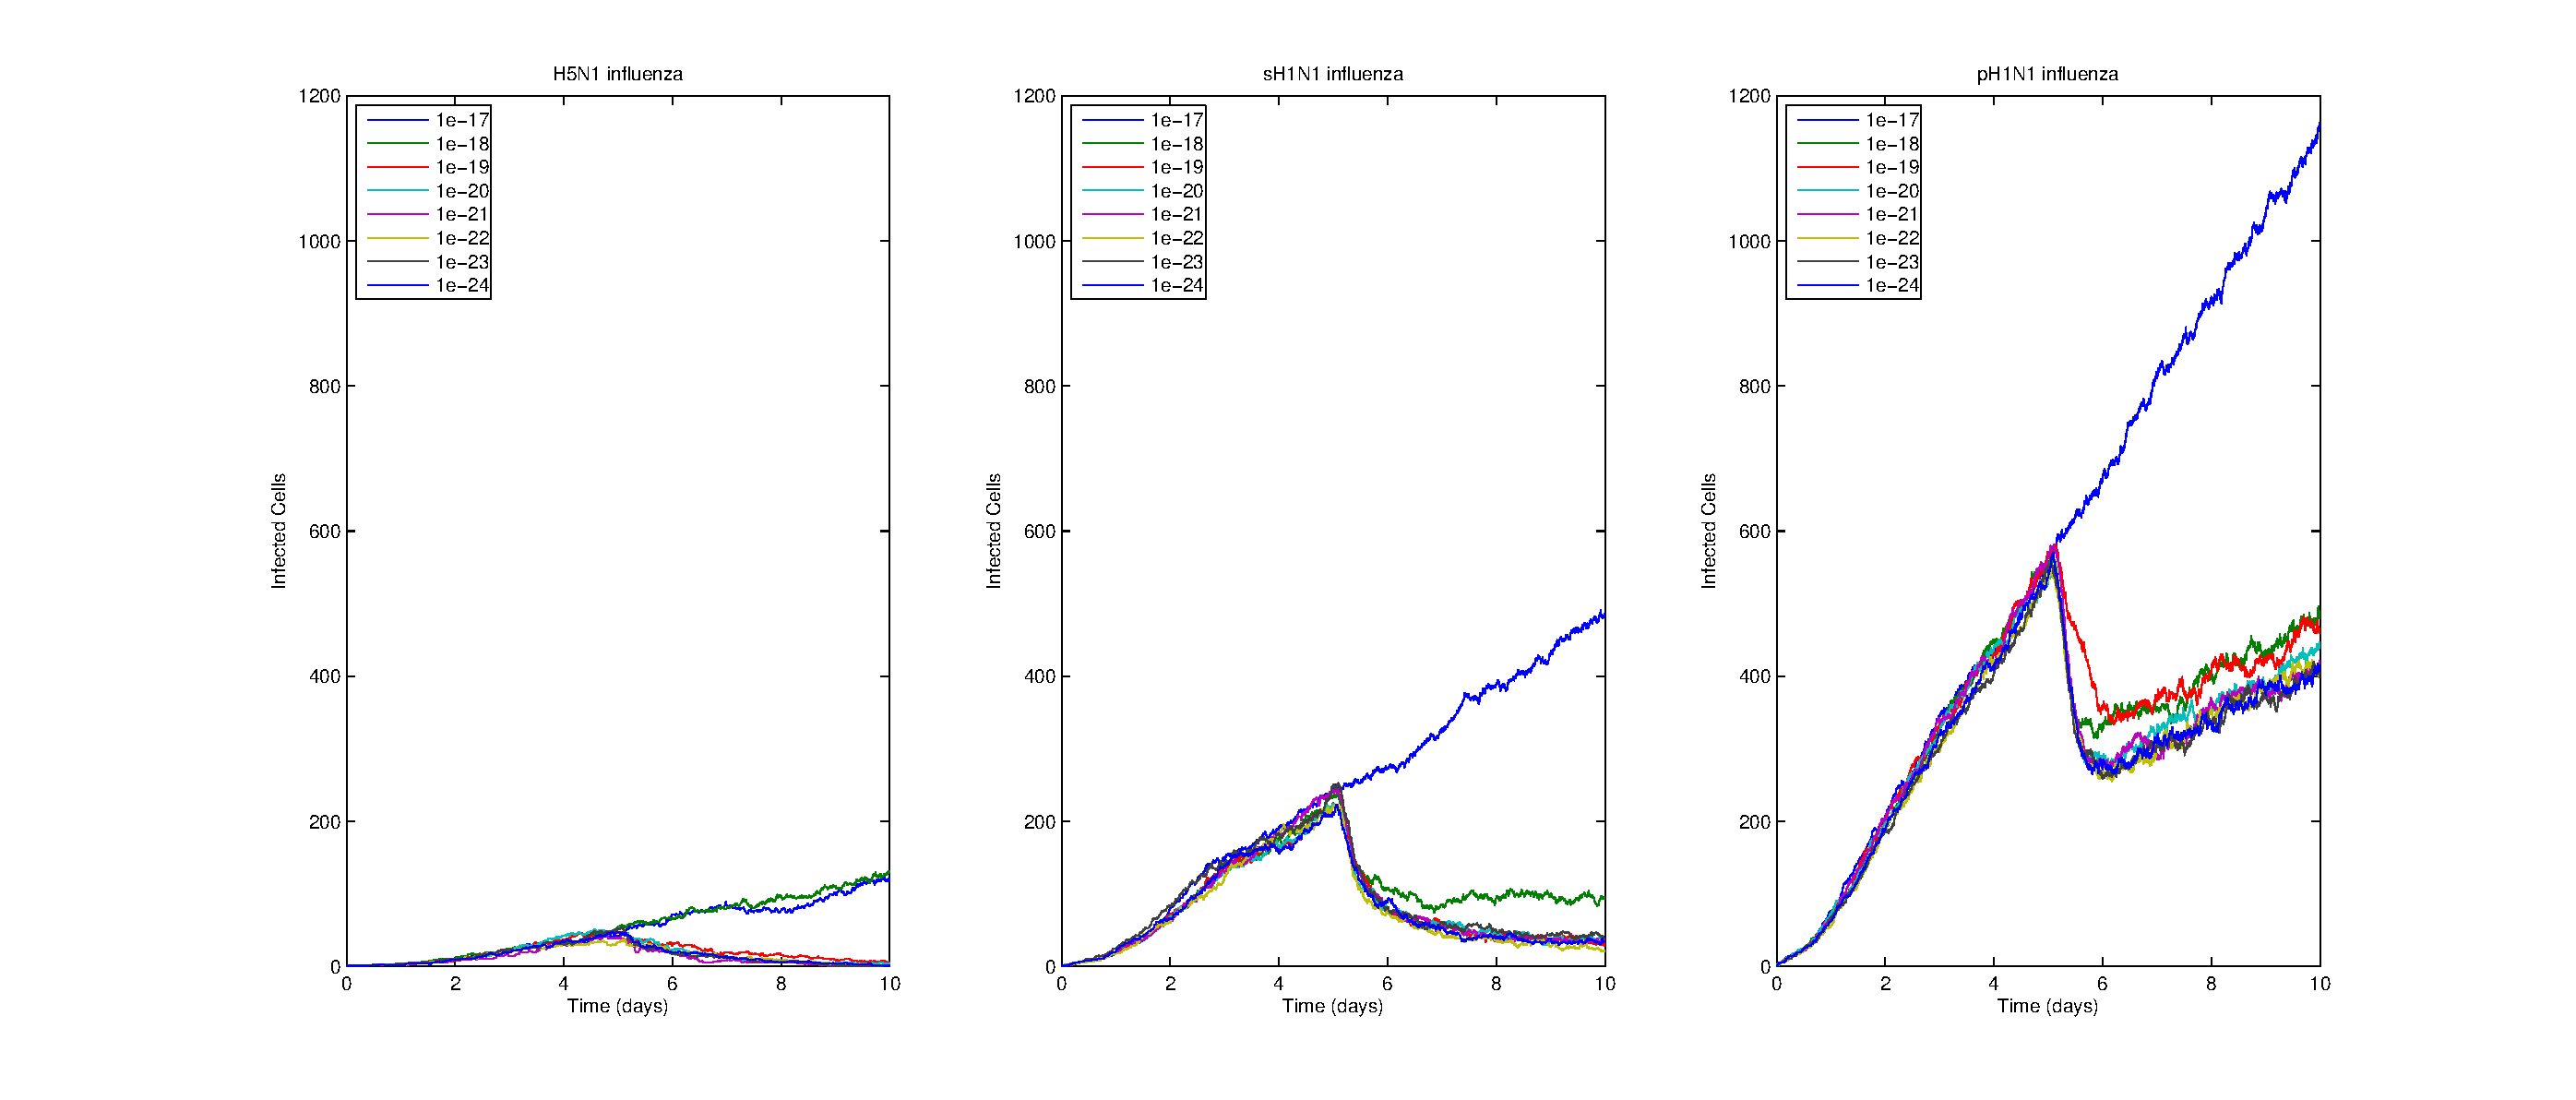
\includegraphics[width=\textwidth]{sensitivity}
 \end{center}
\caption{Varying T-cell sensitivity to chemokine in the model: H5N1 model results use RANTES  only, and sH1N1 and pH1N1 use both IP-10 and RANTES. Total number of infected, expressing and apoptotic cells are plotted for each infection.  The sensitivity value specifies the minimum level of chemokine concentration required for T-cells to detect it. } 
 \label{fig:sensitivity}
\end{figure}


\subsection*{Chemokine combinations}

Because aH5N1 has been shown to suppress the production of interferon \cite{Mitchell2011} we hypothesize that it renders IP-10 ineffectual.  We hypothesize that this leads to the elevated RANTES secretion rates measured in aH5N1 compared to the other two strains (Table~\ref{table:strains}).  Because of this behavior IP-10 was not included in the aH5N1 model runs.

Four models runs were performed for each strain (two for aH5N1) to look at how the presence and/or lack of specific chemokines affect the simulated immune response (Fig.~\ref{fig:chemokine}).  The lack of both chemokines leads to runaway infections in all three strains.  The presence of only RANTES is enough to contain the aH5N1 infection, but is weaker than IP-10 in both H1N1 strains.  IP-10 alone proves to be as effective as the combination of IP-10 and RANTES, suggesting that RANTES does not play a significant role in infections that stimulate an IP-10 response.

\begin{figure}[ht!]
\begin{center}
	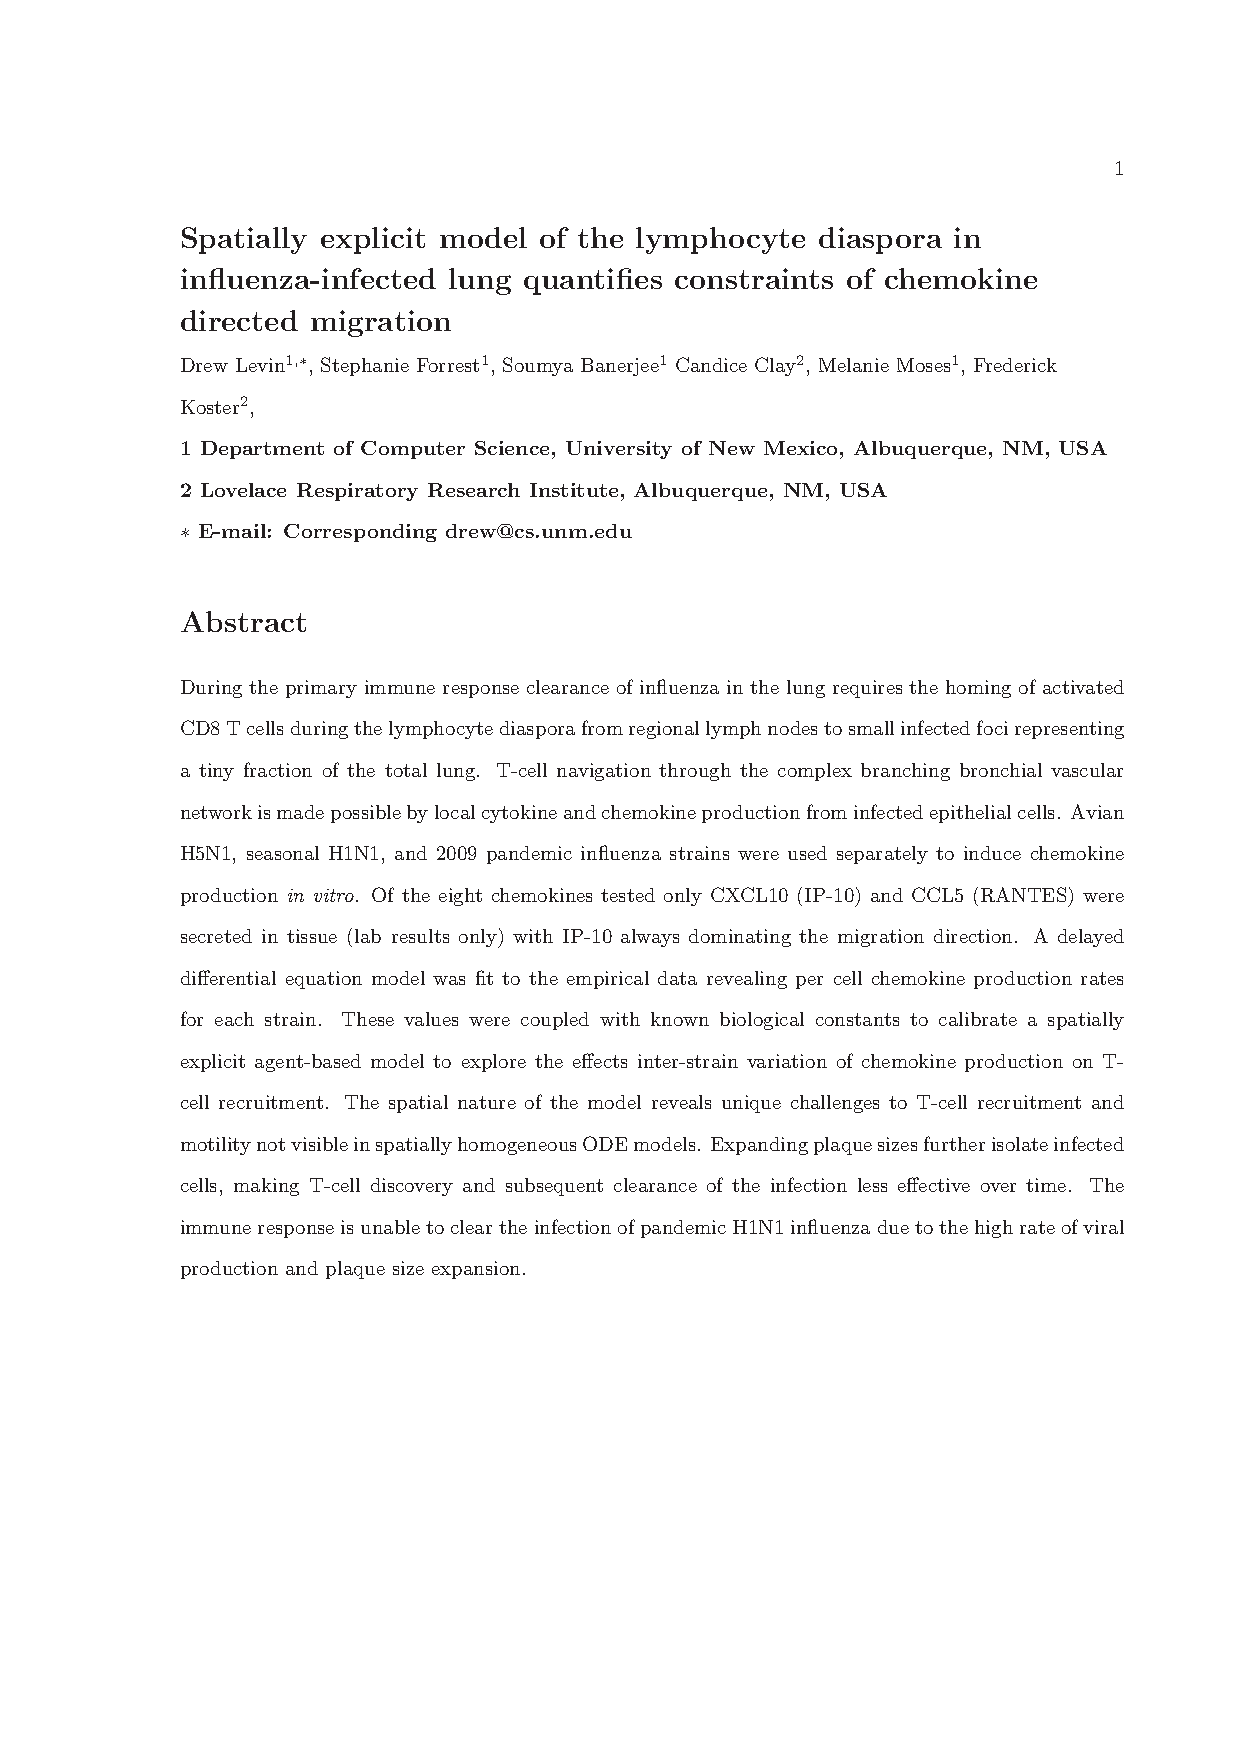
\includegraphics[width=\textwidth]{chemokine}
	\caption{Effects of different chemokine combinations.  A) aH5N1 does not stimulate an IP-10 response.  B-C) sH1N1 and pH1N1 show no significant difference between IP-10 alone versus IP-10 and RANTES combined.}
	\label{fig:chemokine}
\end{center}
\end{figure}



\subsection*{Spatial effects}

Spatial effects of viral and chemokine diffusion play an important role in both the spread and clearance of infection.  Free virus particles diffuse from virus secreting cells and infect healthy cells.  Chemokine produced by infected cells attracts T-cells to the infected cells.  Although virus is produced at a higher rate than chemokine, it diffuses much more slowly because it is a larger particle.  Chemokine diffusion, however, is limited by higher decay rates than the virus.  These countervaling effects result in similar spatial profiles for the two particle types (Fig.~\ref{fig:cycells}).

Early in the infection (up to day 4) the plaque is dominated by active (incubating and secreting) cells, and dead cells are rare. Over time, cells in the plaque's interior die causing active cells to comprise a decreasing proportion of the plaque. T-cells arrive at day 5 and begin to killing the virus-expressing cells. By day 6 a majority of the expressing cells have been eliminated as the plaque becomes dominated by dead cells.  In the H5N1 example the plaque is dense, allowing T-cells to find secreting easily.  Thus the infection can be eliminated.  However, in both H1N1 simulations secreting cells are not eliminated.  In these two cases, expressing cells account for at most 10\% of the active cell population and less than  1\% of the total plaque at 6 days p.i.  T-cells still accumulate, but they arrive at a slower rate than the plaque's rate of growth. This leads to a lower average T-cell killing rate.  Furthermore, the regions of concentrated chemokine lag behind the cell and virus spatial layout.  It takes time for newly secreting cells to produce chemokine and for pockets of high chemokine density to decay.  Thus, T-cells, which rely on the chemokine gradient to find infected cells, often lag behind cellular changes in the plaque.  The delayed response and the low proportion of virus secreting cells prevent T-cells from completely clearing the infection.

\begin{figure}[ht!]
\begin{center}
 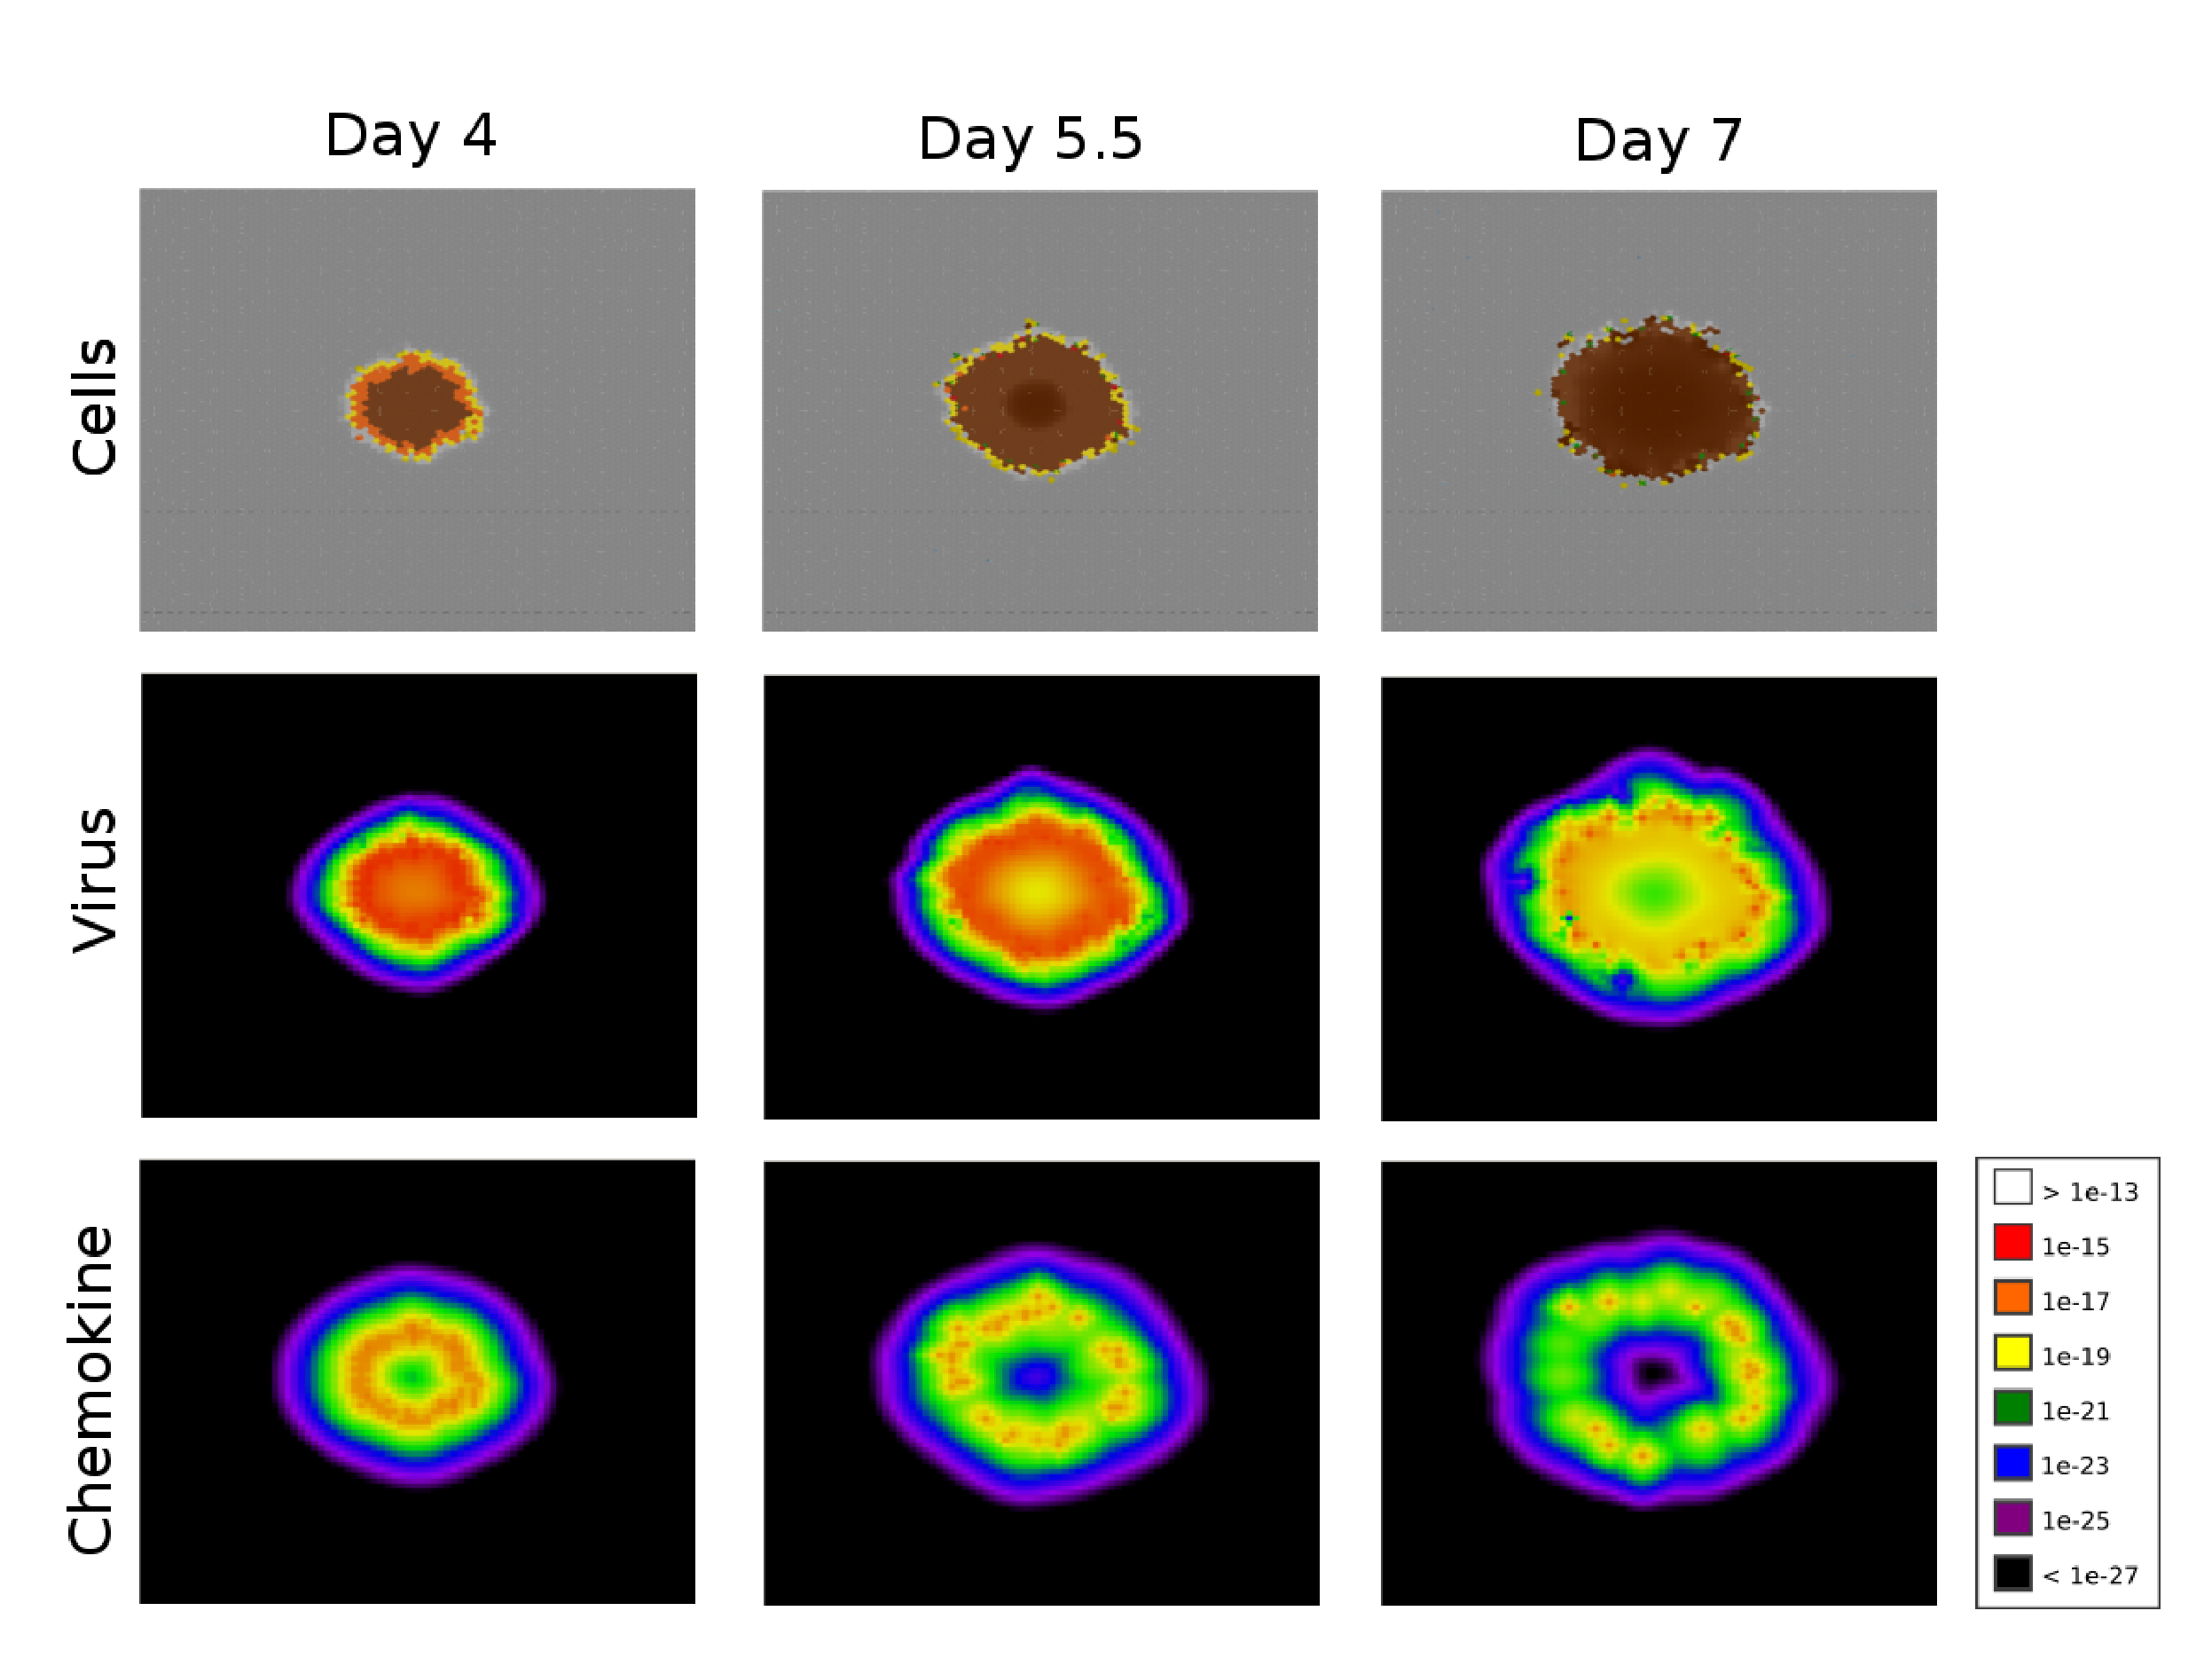
\includegraphics[width=\textwidth]{cycells}
 \end{center}
\caption{Example simulated sH1N1 infection. Screenshots taken at Day 4, Day 5.5, and Day 7.  The top row shows the spreading focus of infection  through the color coding of individual cells:  healthy cells in uninfected tissue (gray),  virus-incubating cells (yellow), virus-secreting cells (orange), apoptotic cells (red), dead cells (brown), and T-cells introduced at day 5 (green).  Free virus and chemokine particles are represented by compartmentalized concentrations of mols/mL and ng/mL (see the legend in the bottom right).} 
 \label{fig:cycells}
\end{figure}


\subsection*{Infection rebound}

The immune response fails to clear sH1N1 completely and is unable to contain pH1N1 (Fig. \ref{fig:variance}).  This appears to be an artifact of the spatial nature of the ABM.  Why can the immune response create an immediate decrease in the number of pH1N1 infected cells at day 5, only to fail in the same endeavor two days later?   Figure \ref{fig:variance} reports only the number of infected cells, not counting dead cells in the focus of infection (FOI).  Further, T-Cells induce apoptosis in virus-secreting cells, but not in virus-incubating cells.  At day 5.5, the ratio of secreting cells to the total number of cells in the FOI is high (Fig.~\ref{fig:cycells}). By day 7, the ratio of secreting cells to total plaque size is approximately 1:100 for both the pH1N1 and sH1N1 strains.  The greater replication rate of pH1N1 widens the gap (Fig.~\ref{fig:plaquesize}C) whereas the lower replication rate of sH1N1 allows the T-cells to control (but not eliminate) the infection.

A cell infected with pH1N1 produces new virus at the rate of 5.08e-3 PFU/s \cite{Mitchell2011}.  That is, a new viral particle is produced approximately every 200 seconds.  Assuming that virus particle secretion continues for one hour after apoptosis is initiated, the best a T-Cell can do is to limit a single infected cell to producing 18 new viral particles.  Without additional immune responses, T-Cells alone cannot contain the pH1N1 infection.  In contrast, the sH1N1 virus-secreting cell produces a new virus particle every 2,643 seconds, allowing a T-cell to limit a single infected cell to 1.3 viral particles in the one-hour window.  Avian H5N1 virus-secreting cells produce only 0.2 viral particles in the interval after T-cell detection. 

\begin{figure}[ht!]
\begin{center}
 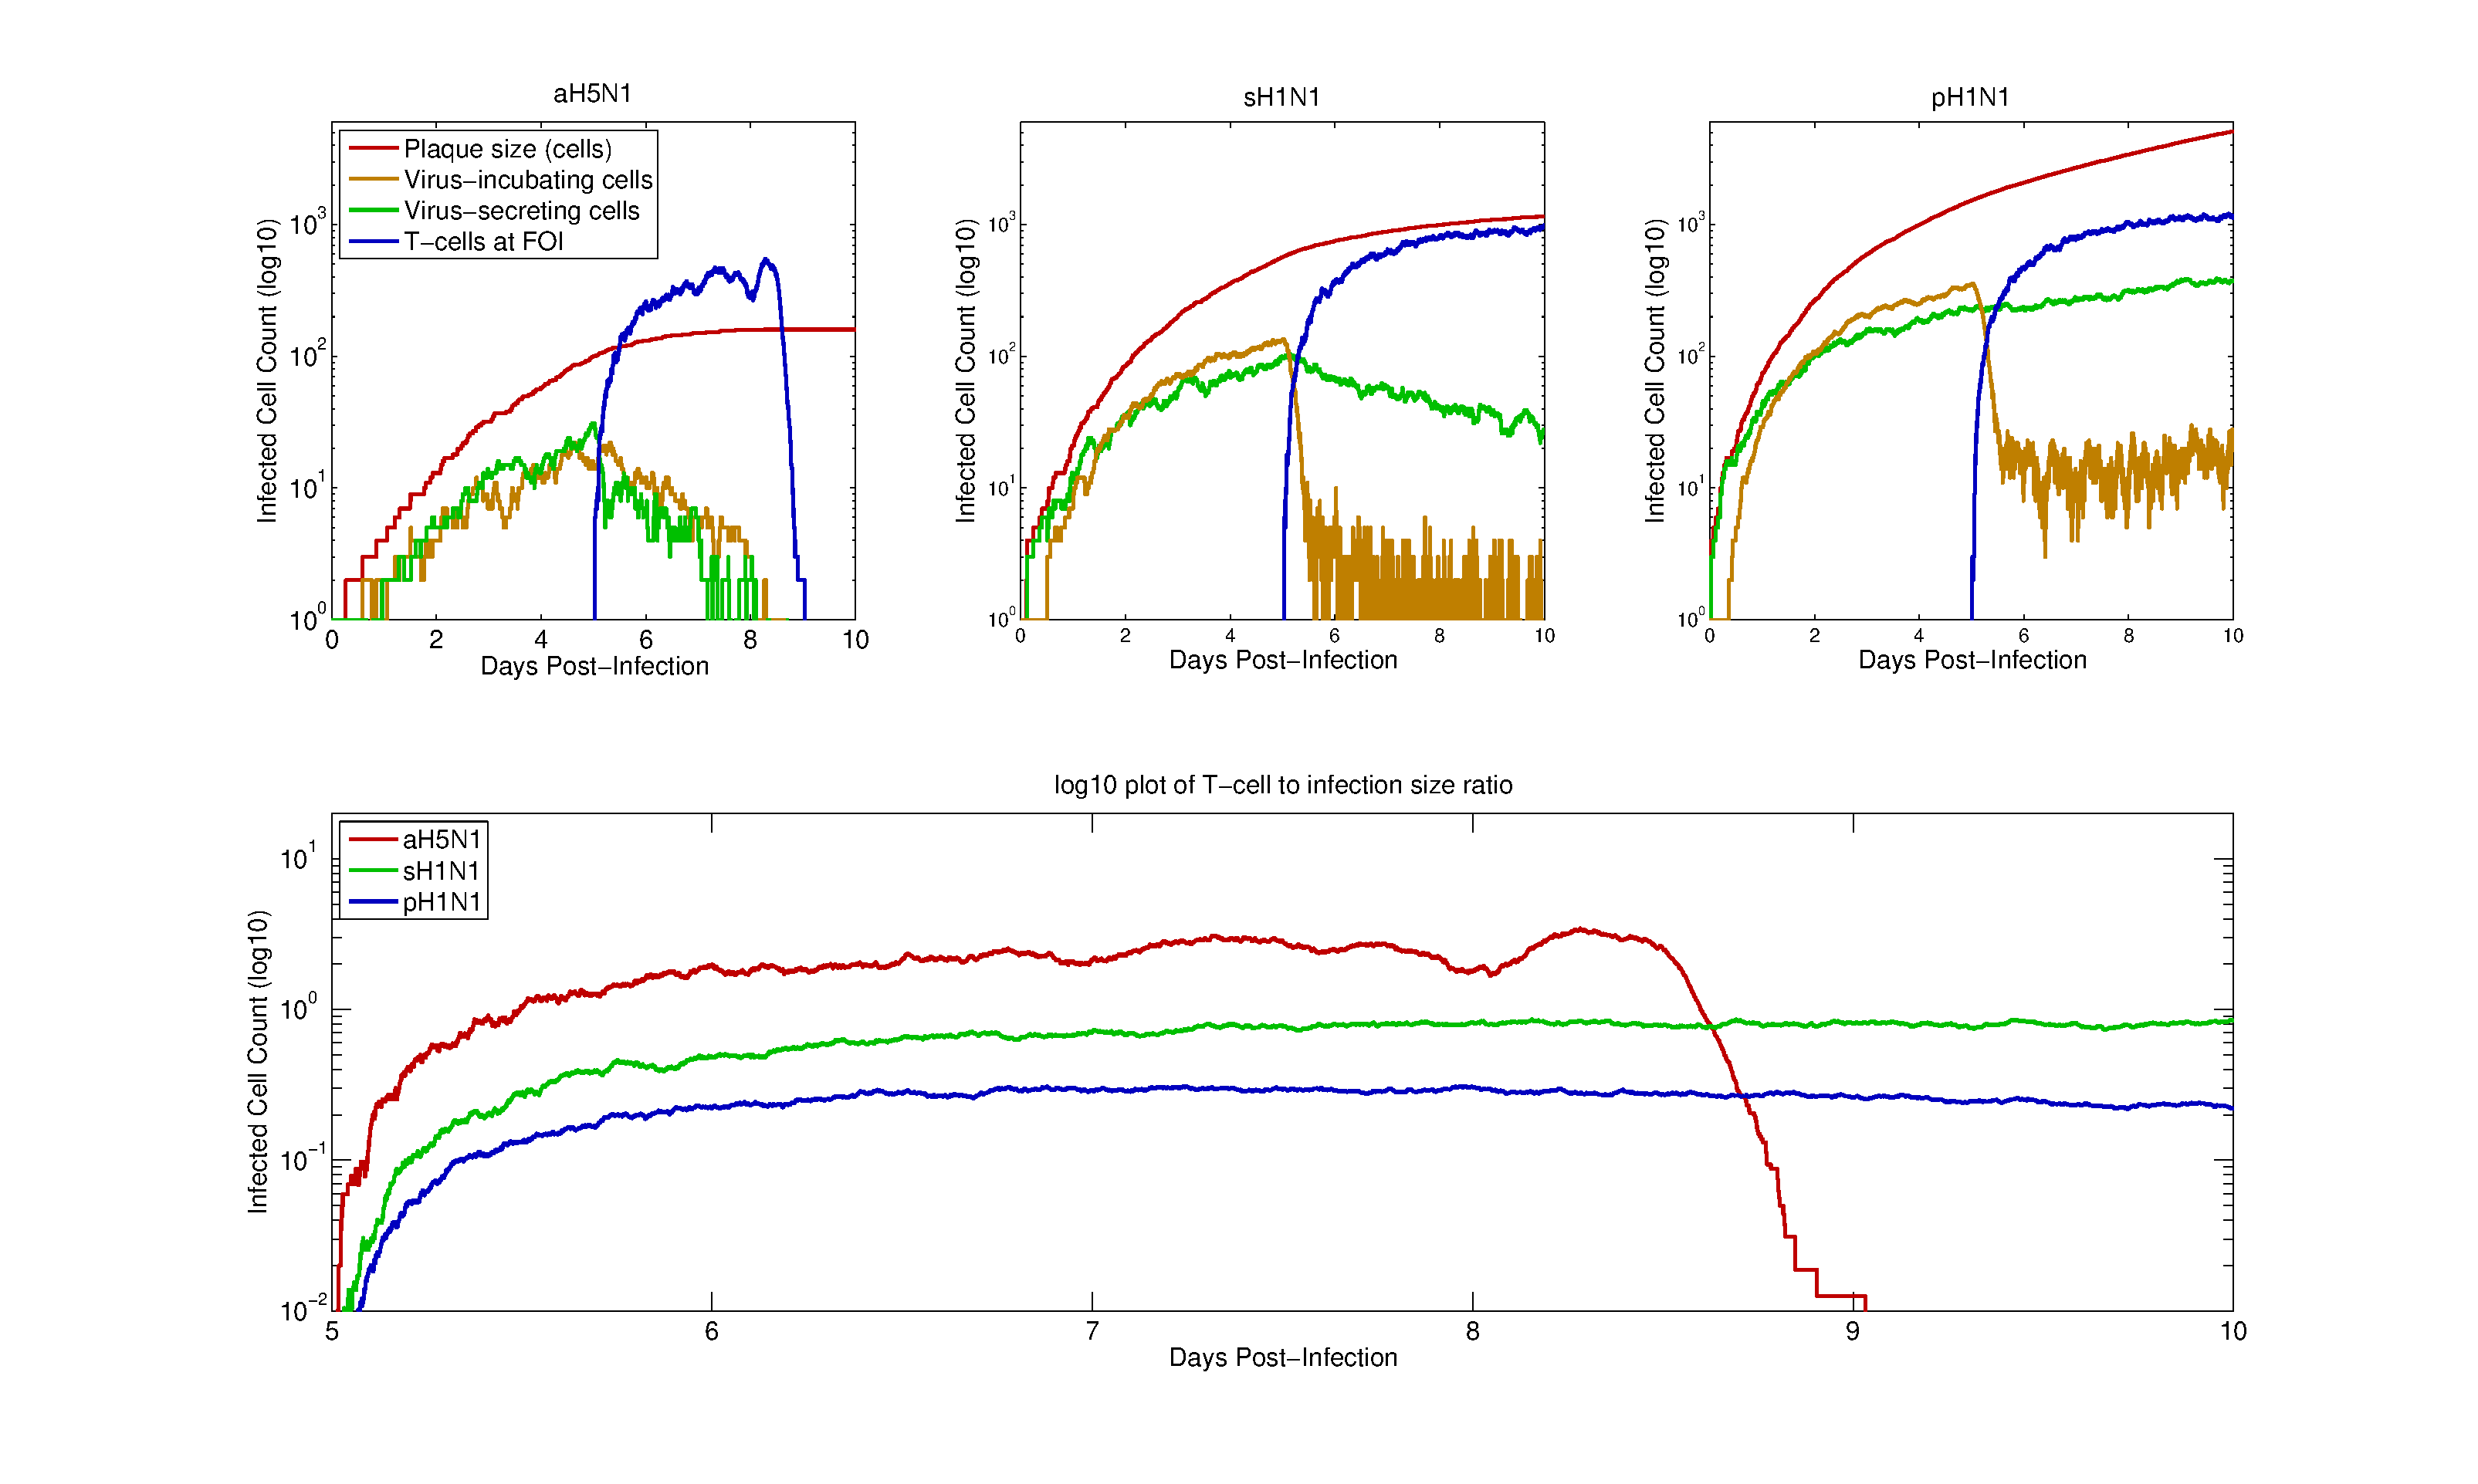
\includegraphics[width=\textwidth]{plaquesize}
 \end{center}
\caption{Comparison of total plaque size (green), number of virus incubating cells (blue), number of virus secreting cells (red), and T-cells (indigo) for the simulated infections of H5N1, sH1N1, and pH1N1.} 
 \label{fig:plaquesize}
\end{figure}


\section*{Discussion}

\subsection*{ABM Advantages}

The use of an ABM has advantages over a spatially homogeneous ODE model.  An ODE model assumes that any virus particle is capable of infecting any healthy cell.  Figure \ref{fig:cycells} shows that this is clearly not the case.  In fact, most free virus exists on top of infected cells that are no longer candidates for viral binding and fusion.  ODE models account for this discrepancy by lowering rates of infection by a constant amount, but this assumes that the proportion of unsuitable virions will always be the same.  This is clearly false as can been seen in Figure~\ref{fig:cycells} where the early infection has a higher proportion of virus overlapping healthy cells.

Another advantage of our ABM is the ability to render the model using OpenGL (Fig.~\ref{fig:cycells}).  The ability to see the model in action reveals spatial dynamics that are absent in ODE models and difficult or impossible to observe in \textit{in vitro} and \textit{in vivo} systems.  For example, observing the simulation reveals challenges to T-cell detection of infected cells that are not apparent using standard population plots.  By watching the model progress, we observed three key phenomena.  First, because T-cells find infected cells by climbing the chemokine gradient, we see T-cell clustering at local maxima of chemokine concentration.  Thus, we have an explanation for why T-cells do not increase in effectiveness as their numbers increase.  Second, we notice that clumps of T-cells remain in place even after all virus-secreting cells have been killed off.  This is because it takes time for the local chemokine maxima to diffuse and decay to a point where the T-cells can once again climb the gradient to a new maxima.  Finally, we can see that infected cells grow more disperse as the size of the infection grows.  Because T-cells cluster together they become incapable of covering the increasing plaque size.  These spatial observations provide explanations for the pH1N1 resurgence that would be hidden without the visualization tools provided by the ABM.

\subsection*{General Immune Response Modeling}

NEW

The adaptive immune response to influenza in the mouse is a complex network of molecular and cellular elements, and incorporation of all of these into a comprehensive predictive model is not yet achieved.  Recent whole-animal models using a data-fitting approach and extensive databases have enhanced our global understanding of response metrics that are difficult or impossible to measure.  We have focused exclusively on the problem of the search of activated CTL for infected foci in the lung, and as in other models have made a number of assumptions.

The generally held view of the sequence of CD8+ T cell events during a primary immune response to influenza in the lung involves the following steps: dendritic cells bearing specific antigen migrate from the lung to the draining lymph node where naïve precursors are encountered and activated.  T cells proliferate in the lymph node and are released into the bloodstream, appearing simultaneous in the lung, spleen and other organs 4-5 days post-infection after to extravasation from the blood [Marshall 2001].   In the lung, extravasation from capillaries is signaled by inflammatory cytokine-mediated integrin-activation on endothelial cells.  Once in the tissue, T cells are guided up a chemokine gradient to the infected epithelial cell secreting the chemokine.  One of the model simplifications we utilized was the equating cytokine and chemokine signals.

A large fraction of the T cells entering lung tissue have come from the spleen where they proliferated under stimulation from antigen-loaded DC.  This has been demonstrated by the significant loss of T cells entering lung following splenectomy differential [Tripp 1997] and by math modeling results that make sense only if there is a significant proliferation of activated cells outside the lymph node prior to arrival in the lung [Wu 2011].  Our model did not include the proliferation in the temporary splenic reservoir as this uncertain degree of time delay in arrival between LN and lung would have complicated our ABM model.  Using numbers of cells egressing from LN likely underestimated the rate of CTL population entering the lung, but our derivations of parameters impacting the T cell search and subsequent function are probably not affected.

The fundamental mechanisms regulating the expansion of viral load and subsequent clearance of virus remain unclear, with current hypotheses focusing on antigen-driven, target cell susceptibility-driven, innate immune response-driven, antigen presentation limited, and adaptive immunity responses.  We used the data from strain-specific viral replication in vitro in human bronchial epithelial cells [Mitchell 2011] to structure the regulation of viral abundance and viral clearance as essentially a model of antigen-driven, innate immunity-driven regulation.  In a differential equation model, regulation of viral load was primarily driven by the availability of susceptible target cells [Baccam 2006].  The question of target-driven versus antigen-driven regulation was addressed in a separate modeling study of infected equine lungs [Saenz 2010], finding that regulation was primarily innate immunity-driven since no more than 27\% of bronchial epithelial cells were ever infected during the course of the lung infection.  In a comprehensive model of murine influenza rate-limiting antigen presentation was the primary influence on viral clearance [Lee 2009].  In a subsequent model based on a large murine database, CD8+ T cells were critical components of the adaptive response in limiting the number of infected cells, with neutralizing antibodies responsible for clearing free virus [Miao 2010].   Most modeling studies used a mouse-adapted virus to enable enumeration of epitope-specific T cells, making direct comparisons of replication efficiency with our human virus isolates more difficult.  The mechanism of regulation of animal viral load may be specific to viral replication efficiencies, strain-specific suppression of innate immunity, and the phase of the immune response.  We compared the three strains for their demands placed on the T cell search mechanism to find and kill infected cells. The multiplicity of potential regulation mechanisms does not invalidate our approach to the T cell search mechanisms. 

Our focus on the T cell search necessitated the simplification or removal of selected features of the mammalian immune response, in order to permit tractable simulations.  Antigen presentation and peripheral lymphoid tissue amplification of the T cell clonal response is represented solely by the constant rate of emigration of activated T cells from regional lymph nodes.  Virus-specific strain replication rates are represented as constant rates, and virus clearance is also constant.  The contribution of IgM antibody clearing free virus is represented at a constant rate, and the class switch to higher affinity antibody mediated by CD4+ T cells is not represented.  All of these rates may in fact be time-variable rates as indicated by superior data-fitting models [Wu 2011].  Immigration and contributions of virus-nonspecific immune cells such as macrophages are not represented in our model.  Finally, the proliferation of activated T cells in lung tissue is not represented, but is thought to be crucial in the control of lung infection [Miao 2010].  Since known critical components were omitted or simplified, our model was not designed to demonstrate clearance of virus from the lung.  Rather our goal was to examine the features of the response that permitted T cells to sense and contact infected target cells.


\subsection*{Chemokine Directed T-cell Search}

Hypercytokinemia is a characteristic of virulent influenza strains \cite{DeJong2006} but bloodstream levels of cytokines and chemokines may not reflect local concentrations and dynamics critical in guiding T cells to infected epithelial cells.  We elected to use our data on in vitro secretion of chemokines by human bronchial epithelial (NHBE) cells obtained from the same cultures of the three virus strains previously reported \cite{Mitchell2011}.  In this study the replication kinetics and productivity of the three virus strains were markedly different, but monolayer infection was initiated with a low MOI of 0.01 or 0.001, mimicking the initial infection naturally.  The levels of the chemokines CCL5 and CXCL10 in the basal media induced by the 3 strains were approximately equivalent at 24h post-infection.  When the productivity per cell was calculated, the avian H5N1 strain induced higher secretion of CCL5 (RANTES) than the seasonal or pandemic strains.  Greater CCL5 secretion by H5N1 strains has been noted in in vitro NHBE cultures when a relatively high MOI is used compared to seasonal strains \cite{Chan2005, Chan2010, Zeng2011} and pandemic strains \cite{Zeng2011}.  MOI and degree of differentiation of NHBE are critical determinants of cyto/chemokine secretion \cite{Chan2010}.  However, in spite of the attenuated type 1 interferon response induced by H5N1 strains \cite{Zeng2007}, the chemokine secretion is not attenuated.

Chemokines with a clear role directing T cell traffic include CXCL10 \cite{Dufour2002}, CCL5 \cite{Kawai1999} and CCL3 \cite{Kawai1999}.  The chemokine receptor CCR5, binding CCL5 and other chemokines, is crucial in the accelerated recruitment of CD8+ T cells to lung airways \cite{Kohlmeier2008}.  Other chemokines are likely to play a role in T cell traffic.  Although we did not detect significant levels of other chemokines in our cultures, the neutrophil- and T cell-attractant CXCL8/IL-8 is secreted into seasonal influenza-infected NHBE cultures \cite{Matsukura1996, Arndt2002}.  In the intact animal immigrant inflammatory cells particularly macrophages augment the multiple chemokine signals \cite{Julkunen2000}.  Finally, antigen-specific CD8+ T cell recognition of its target will induced lung injury mediated by TNFa and trigger addition alveolar epithelial cell chemokine secretion \cite{Zhao2000}.   Thus our model represents only a portion of the complete chemokine signal complex operating in the infected animal.

A key determinant in the efficiency of chemokine-directed T cell migration towards virus-secreting epithelial cells is the communication distance, defined by the threshold of sufficient chemokine signal to induce directed motion of the cell up the chemical gradient \cite{Thelen2008}.  The diameter of this cloud generated by a single cell is a function of production rate, decay rate, protein diffusion and the sensitivity threshold.  For the threshold of 100 pg/mL and maximal levels of concentration in tissue of 10,000 pg/mL, we calculated the effective communication distance as approximately 250 microns in our model.  This calculation matches the distance calculated for generic cytokines secreted by a suspended solitary cell \cite{Francis1997}.

NEW

In our model directed migration and viral infection control was not limited over a wide range of T cell sensitivity to the chemotactic signal.  The density of CCR5 receptors on the surface of CD8+ T cells was a determinant of the strength of chemotactic attraction for CCR5 ligands such as CCL5 in an in vitro assay [Desmetz 2006].   The density of CCR5 receptors on human CD8+ T cells vary over an order of magnitude, suggesting that sensitivity to the chemotactic signal could play a role in susceptibility to infection.  CCR5-knockout mice are susceptible to fatal Cryptococcal encephalitis/meningitis [Huffnagle 1999] and West Nile virus encephalitis [Glass 2005].  In the Cryptococcus-infected mice T cell recruitment to the brain, but not to the lung, was impaired.   In CCR5-KO mice influenza A virus pneumonia was more severe associated with decreased T cell recruitment to the lung, while in CCR2-KO mice decreased T cell recruitment was due to decreased macrophage influx into the lung [Dawson 2000].  On the other hand, CCL5-KO mice and CXCR3-KO mice (the receptor for CXCL10/IP-10) had similar viral kinetics and leukocyte recruitment compared to the wild-type mice [Wareing 2004].  Finally, humans with the CCR5-D32 deletion allele may have increased susceptibility to the pandemic 2009 H1N1 influenza in a small sample [Keynan 2010].  The question of limiting sensitivity has practical implications, since immunomodulation of cytokine/chemokine signaling to decrease influenza mortality is currently under investigation [Oslund 2011; Alleva 2011; Bassaganya-Riera 2010; Budd 2007; Moseley 2010].  While blocking chemokine function may decrease inflammation and death from viral pneumonia, it may have an unintended consequence of impairing adaptive immunity.  Thus, specific T cell recruitment to the influenza virus-infected lung should be quantitatively assessed in chemokine receptor-knockout mice.

\subsection*{Caveats and Limitations}

In both H1N1 strains the T-cell response fails to clear the infection by day 10.  In the case of pandemic H1N1, the infection continues to accelerate after a short period of clearance.  We suggest that this is due to the absence of several innate immune agents that were not included in the model.  We chose to remove most of the innate response in order to better focus on the relative effects of the cytokine signaling and T-cell response.  Although the infections do not clear by day 10, the models show clear differences in the ability of the immune system to deal with influenza strains of varying replication rates.  We see that the viral production rate is a major factor in the strength of the infection.

Our model combines the dynamics of human epithelial tissue with the scaling of a mouse's immune system.  We choose to use mouse scale models because of the computational limitations of our ABM.  By limiting our model to mice, we are able to keep the active agent population below 100,000, which allows a single model to be run in less than a day.  A human-sized model would be computationally intractable.  We find this practice acceptable for two reasons.  First, the size differences and scaling principles between mice and human has been well documented [REF?] and can be accounted for.  Second, this paper focuses on relative differences between strains so an exact recreation of the immune response is not necessary.

In our model, the ability of T-cells to detect a chemokine signal and their subsequent motility upon doing so rests entirely on the T-cell's sensitivity to chemokine parameter.  Once a T-cell encounters a concentration of chemokine above the sensitivity threshold it will immediately climb the chemotactic gradient to the local maxima.  Studies of T-cell chemotaxis show that T-cell movement depends more on the magnitude of the chemokine gradient rather than the concentration \cite{Gao2003}.  Furthermore, T-cells will perform a biased random walk rather than moving in a straight line directly up the concentration gradient [REF?].  We experimented with biased random walks in our model and noticed no change in any results.  Thus, we chose to keep the model simple and limited T-cell movement to directly climbing the chemokine gradient.

% Do NOT remove this, even if you are not including acknowledgments
\section*{Acknowledgments}


\section*{References}
% The bibtex filename
\bibliography{references}

\section*{Figure Legends}
%\begin{figure}[!ht]
%\begin{center}
%%\includegraphics[width=4in]{figure_name.2.eps}
%\end{center}
%\caption{
%{\bf Bold the first sentence.}  Rest of figure 2  caption.  Caption 
%should be left justified, as specified by the options to the caption 
%package.
%}
%\label{Figure_label}
%\end{figure}


\section*{Tables}
%\begin{table}[!ht]
%\caption{
%\bf{Table title}}
%\begin{tabular}{|c|c|c|}
%table information
%\end{tabular}
%\begin{flushleft}Table caption
%\end{flushleft}
%\label{tab:label}
% \end{table}

\end{document}

